% vim: set textwidth=78 autoindent:

%\subsection{Delimited Text Plugin}\label{label_dltext}    
\subsection{Extension Texte Délimité}\label{label_dltext}    

% when the revision of a section has been finalized, 
% comment out the following line:
%\updatedisclaimer

%The Delimited Text plugin allows you to load a delimited text file as a layer in QGIS. 
L'extension Texte Délimité permet de charger un fichier texte délimité comme 
couche dans QGIS. 

%\minisec{Requirements}
\minisec{Exigences}

%To view a delimited text file as layer, the text file must contain:
Pour afficher un fichier texte délimité comme une couche, le fichier texte 
doit contenir :

%\begin{enumerate}      
%\item A delimited header row of field names. This must be the first line in the text file.
%\item The header row must contain an X and Y field. These fields can have any name.
%\item The x and y coordinates must be specified as a number. The coordinate system is not important.
%\end{enumerate}
\begin{enumerate}      
\item Une ligne d'en-tête délimité contenant les noms des champs. Cette ligne 
doit être la première du fichier.
\item La ligne d'entête doit contenir les champs X et Y. Ces champs peuvent 
avoir n'importe quel nom.
\item Les coordonnées X et Y doivent être de type numérique. Le système de 
coordonnées n'est pas important.
\end{enumerate}

%As an example of a valid text file we import the elevation point data file 
%\filename{elevp.csv} coming with the QGIS sample dataset (See Section~\ref{label_sampledata}):
Comme exemple de fichier texte valide, nous pouvons importer le fichier point 
d'élévation \filename{elevp.csv} fourni avec le jeu de données échantillon de 
QGIS (voir la Section~\ref{label_sampledata}):

\begin{verbatim} 
X;Y;ELEV
-300120;7689960;13
-654360;7562040;52
1640;7512840;3
[...]
\end{verbatim}

%Some items of note about the text file are:
Nous noterons les points suivants à propos du fichier texte :

%\begin{enumerate}
%\item The example text file uses \mbox{$;$} as delimiter. Any character can be used to delimit the fields.
%\item The first row is the header row. It contains the fields X, Y and ELEV.
%\item No quotes ({\tt{}"{}}) are used to delimit text fields.
%\item The x coordinates are contained in the {\em X} field.
%\item The y coordinates are contained in the {\em Y} field.
%\end{enumerate}
\begin{enumerate}
\item Le fichier texte d'exemple utilise le \mbox{$;$} comme délimiteur. 
N'importe quel caractère peut être utilisé comme délimiteur de champ.
\item La première ligne est la ligne d'entête. Elle contient les champs X, Y 
et ELEV.
\item Les guillemets ({\tt{}"{}}) ne peuvent pas être utilisés pour délimiter 
les champs textes.
\item Les coordonnées x sont incluses dans le champ {\em X}.
\item Les coordonnées y sont incluses dans le champ {\em Y}.
\end{enumerate}

%\minisec{Using the Plugin}
%To use the plugin you must first enable it as described in Section \ref{sec:managing_plugins}.
\minisec{Mettre en oeuvre l'extension}
Pour utiliser l'extension, vous devez d'abord l'activer comme décrit dans la 
Section \ref{sec:managing_plugins}.

%Click the new toolbar icon \toolbtntwo{delimited_text}{Add Delimited Text Layer} to open the Delimited Text dialog as shown in Figure \ref{fig:delim_text_plugin_dialog}.
Appuyez sur la nouvelle icône apparue dans la barre d'outils \toolbtntwo{delimited_text}{Ajoutez un fichier de texte sur la couche} 
pour ouvrir la boîte de dialogue Texte Délimité comme montré dans la Figure \ref{fig:delim_text_plugin_dialog}.

%\begin{figure}[ht]
%   \begin{center}
%   \caption{Delimited Text Dialog \nixcaption}\label{fig:delim_text_plugin_dialog}\smallskip
%   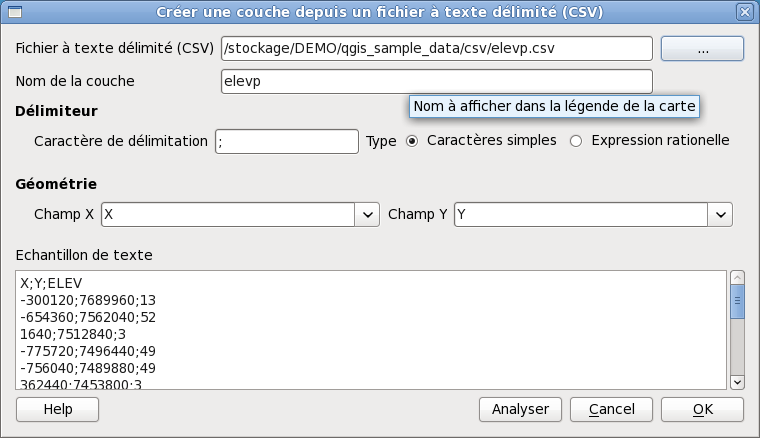
\includegraphics[clip=true, width=9cm]{delimited_text_dialog}
%   \end{center}  
%\end{figure}
\begin{figure}[ht]
   \begin{center}
   \caption{La boîte de dialogue Texte Délimité \nixcaption}\label{fig:delim_text_plugin_dialog}\smallskip
   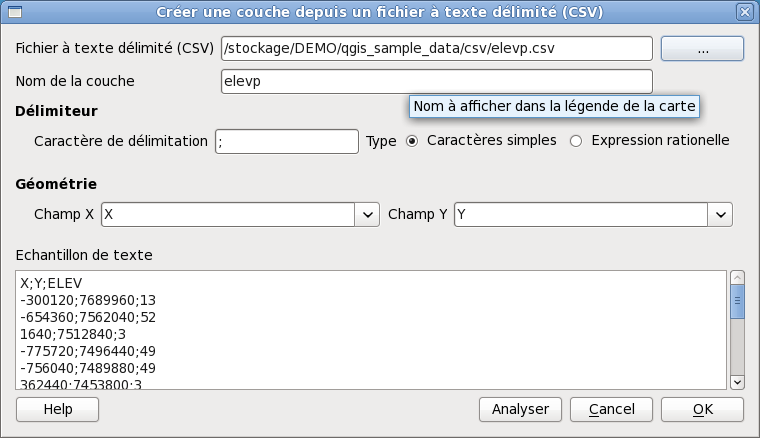
\includegraphics[clip=true, width=9cm]{delimited_text_dialog}
   \end{center}  
\end{figure}

%First select the file (e.g., \filename{qgis\_sample\_data/csv/elevp.csv}) to import by clicking 
%on the \button{Browse} button. Once the file is selected, the plugin attempts to parse the file 
%using the last used delimiter, in this case a semi-colon (\mbox{$;$}). To properly parse the file, it 
%is important to select the correct delimiter. To change the delimiter to tab use 
%\mbox{$\backslash$}t (this is a regular expression for the tab character).
%After changing the delimiter, click \button{Parse}.
Sélectionnez d'abord le fichier à importer (par exemple, \filename{qgis\_sample\_data/csv/elevp.csv}) 
en appuyant sur le bouton \button{Parcourir...}. Une fois le fichier 
sélectionné, l'extension essaie d'analyser le fichier en utilisant le dernier 
délimiteur utilisé, dans le cas présent le point-virgule (\mbox{$;$}). 
Afin d'analyser correctement le fichier, il est important de sélectionner le 
bon délimiteur. Pour changer et utiliser le délimiteur tabulation, utilisez \mbox{$\backslash$}t 
(c'est l'expression en vigueur pour indiquer le caractère tabulation).
Après avoir changé le délimiteur, appuyez sur \button{Analyser}.

%Once you have parsed the file, choose the X and Y fields from the drop down lists and 
%enter a Layer name (e.g., \filename{elevp} ) as shown in Figure 
%\ref{fig:delim_text_plugin_dialog}. To add the layer to the map, click 
%\button{Add Layer}. The delimited text file now behaves as any other map layer in QGIS.
Une fois le fichier analysé, choisissez les champs X et Y à l'aide des listes 
déroulantes et choisissez un nom de couche (par exemple, \filename{elevp} ) 
comme montré dans la Figure \ref{fig:delim_text_plugin_dialog}. Pour ajouter 
la couche à la carte, appuyez sur \button{OK}. Le fichier texte délimité se 
comporte maintenant dans QGIS comme n'importe quelle autre couche de la carte.
